\section{}
\textit{Provide a clean vector plot of the flow velocity that clearly illustrates the mixing of two
streams of air. Particularly, what do these vector results indicate about the flow physics?
Use screenshots and other illustrations to support your statement.}

\subsection*{Solution}
\begin{figure}[h]
    \centering
    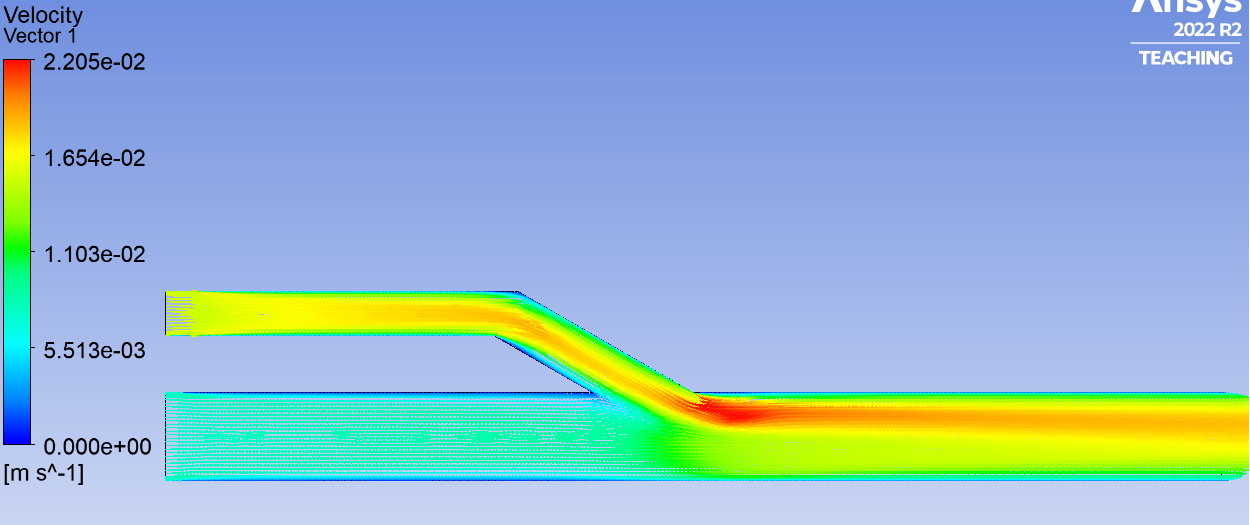
\includegraphics[width=0.8\textwidth]{Questions/Figures/velocity vector.png}
    \caption{Vector field plot of the flow velocity}
    \label{fig:contour}
\end{figure}

The velocity plot shows much of the same information as the contour plot. The plot clearly illustrates the mixing of two streams of air. The plot indicates that the higher velocity flow `pushes' down the lower velocity field. As the flow continues, the stream seems to `mix' the velocities to an average velocity as it approaches the outlet.

For both the upper and lower flows, a boundary layer can be seen developing starting from the inlet. The boundary layer is more pronounced for the upper flow.

Also, the velocity of the upper stream increases around the corner where the flows mix.